\section{Χαρακτηριστικά που υλοποιήθηκαν} \label{section:4-5-implemented-parts}

Όπως αναλύθηκε στο προηγούμενο κεφάλαιο, κατά την υλοποίηση εμφανίστηκαν διάφορα προβλήματα που δεν είχαν προβλεφθεί και τα οποία προκάλεσαν καθυστερήσεις στην ολοκλήρωση των tasks. Λόγω των καθυστερήσεων αυτών έγιναν διάφορες αναδιαμορφώσεις του προγραμματισμού των Sprint καθώς και διαπραγματεύσεις της σημαντικότητας των χαρακτηριστικών. Από τον επανασχεδιασμό και τις προσαρμογές αυτές προέκυψαν μερικές αλλαγές στο τελικό σετ των χαρακτηριστικών της πλατφόρμας σε σχέση με ό,τι είχε αρχικά προδιαγραφεί.

Τα χαρακτηριστικά και οι αντίστοιχες Λειτουργικές Απαιτήσεις που τελικά υλοποιήθηκαν είναι:

\begin{itemize}
    \item Η εγγραφή χρήστη και η δημιουργία των τοπικών βάσεων του, όπως περιγράφονται στις \ref{srs:functional-srs-sign-up} \& \ref{srs:functional-srs-create-user-databases} και στο σενάριο χρήσης \ref{subsection:3-6-use-case-signup}.
    \item Η αυτόματη είσοδος χρήστη, όπως περιγράφεται στη \ref{srs:functional-srs-sign-in} και στο σενάριο χρήσης \ref{subsection:3-6-use-case-signin}.
    \item Η δημιουργία θέματος και η δημιουργία ψηφοφοριών, όπως περιγράφονται στις \ref{srs:functional-srs-create-topic} \& \ref{srs:functional-srs-create-polls} και στο σενάριο χρήσης \ref{subsection:3-6-use-case-create-topic}.
    \item Η περιήγηση στα υπάρχοντας θέματα, όπως περιγράφεται στη \ref{srs:functional-srs-browse-community-topics} και στο σενάριο χρήσης \ref{subsection:3-6-use-case-fetch-topic}.
    \item Η δημοσίευση μηνύματος, όπως περιγράφεται στη \ref{srs:functional-srs-create-post} και στο σενάριο χρήσης \ref{subsection:3-6-use-case-create-post}.
    \item Η επεξεργασία μηνύματος, όπως περιγράφεται στη \ref{srs:functional-srs-modify-post} και στο σενάριο χρήσης \ref{subsection:3-6-use-case-modify-post}.
    \item Η ψήφιση σε ψηφοφορία, όπως περιγράφεται στη \ref{srs:functional-srs-vote-polls} και στο σενάριο χρήσης \ref{subsection:3-6-use-case-vote-in-poll}.
    \item Η ψήφιση σε μηνύματα, όπως περιγράφεται στη \ref{srs:functional-srs-vote-posts} και στο σενάριο χρήσης \ref{subsection:3-6-use-case-vote-post}.
    \item Η διαγραφή των τοπικών δεδομένων, όπως περιγράφεται στη \ref{srs:functional-srs-delete-local-data} και στο σενάριο χρήσης \ref{subsection:3-6-use-case-delete-local-data}.
\end{itemize}

Τα παραπάνω αντιστοιχούν σε 11 ολοκληρωμένες από τις 13 προδιαγεγραμμένες ΛΑ ή πλήρωση 84.6\%, ποσοστό που θεωρείται από τους συγγραφείς επαρκές για την εξαγωγή συμπερασμάτων για τον χώρο των DApps και υπερβάλλον για τα πλαίσια ενός PoC. Στο παράρτημα \ref{appendix-a} παρατίθενται τα στιγμιότυπα οθόνης των υλοποιημένων χαρακτηριστικών.

Το χαρακτηριστικό το οποία παραλήφθηκε είναι η δημιουργία κοινοτήτων και ο ορισμός εξωτερικών contracts για τα tokens τους, όπως περιγράφονται στις \ref{srs:functional-srs-create-communities} \& \ref{srs:functional-srs-assign-community-contract} και στο σενάριο χρήσης \ref{subsection:3-10-use-case-create-community}.

Όσον αφορά στις Μη Λειτουργικές Απαιτήσεις, η \ref{srs:non-functional-srs-maximum-decentraliztion}, η οποία απαιτεί τη μεγιστοποίηση της αποκέντρωσης της πλατφόρμας, εκπληρώθηκε σε ικανοποιητικό βαθμό, παρότι φαινομενικά το σύστημα περιλαμβάνει σημεία κεντροποίησης για ορισμένες λειτουργίες του. Ενώ, δηλαδή, η διάθεση του frontend της εφαρμογής και των contract artifacts, καθώς και η διαδικασία ανακάλυψης των IPFS peers πραγματοποιούνται μέσω υπηρεσιών που εκτελούνται σε κεντρικούς εξυπηρετητές, στην πραγματικότητα είτε απλά παρέχουν σημαντικές διευκολύνσεις στο περιβάλλον ανάπτυξης, είτε αποτελούν προσωρινά εμπόδια που σχετίζονται με τους τρέχοντες περιορισμούς των υποκείμενων τεχνολογιών. Έτσι, από τη μία πλευρά ο κώδικας της εφαρμογής είναι εφικτό να διατίθεται στους χρήστες με αποκεντρωμένο τρόπο (π.χ. μέσω του ίδιου του IPFS), από την άλλη η παρούσα ανάγκη ύπαρξης των rendezvous server για το peer discovery μένει να επιλυθεί από την προγραμματιστική ομάδα του IPFS.

Επίσης, η ΜΛΑ που αφορά στην ελαχιστοποίηση των fees (\ref{srs:non-functional-srs-minimize-fees}) ακολουθήθηκε κατά το δυνατόν σε ολόκληρες τις διαδικασίες του σχεδιασμού και της υλοποίησης. Αυτό επιτεύχθηκε τόσο με την αποθήκευση των απολύτως απαραίτητων δεδομένων επί του blockchain, όσο και με τη βελτιστοποίηση του κώδικα των smart contracts, ώστε να εκτελείται με τον μικρότερο δυνατό αριθμό υπολογιστικών κύκλων.

Τέλος, η ΜΛΑ που σχετίζεται με την αναβαθμισιμότητα των contracts (\ref{srs:non-functional-srs-upgrade-contracts}) καταστρατηγήθηκε, λόγω του επιπρόσθετου χρόνου που θα απαιτούσε μία τέτοια υλοποίηση. Ωστόσο, υπάρχουν ήδη πλήρως λειτουργικές μέθοδοι για την επίτευξη αυτού του στόχου, με διαθέσιμα plugin\footnote{\url{https://docs.openzeppelin.com/upgrades-plugins/1.x/}} που μπορούν να ενσωματωθούν απευθείας στις υπάρχοντες ροές εργασίας.

\subsection{Διαφορές σχεδιασμού-υλοποίησης} \label{subsection:4-5-1-design-implementation-differences}

Σημαντικές διαφορές υπήρξαν επίσης στην διαδικασία υλοποίησης τόσο όσον αφορά στον αριθμό και στις λειτουργίες των διαφορετικών πακέτων λογισμικού όσο και τον χρονοπρογραμματισμό. Προστέθηκαν τρεις νέες υπηρεσίες, η υπηρεσία "Concordia Contracts Provider", ο προσαρμοσμένος IPFS pinner "Concordia Pinner" και η ιστοσελίδα "Concordia Guide".

Η ανάγκη για τα νέα πακέτα λογισμικού προέκυψε κατά την πορεία υλοποίησης της διπλωματικής και προστέθηκαν στον χρονοπρογραμματισμό που είχε γίνει στην αρχή της εργασίας. Στην προσαρμογή αυτή βοήθησαν ιδιαίτερα οι Agile τακτικές που ακολουθήθηκαν και η προσαρμοστικότητα που προσφέρει το Scrum σε μεταβαλλόμενες απαιτήσεις.

Τέλος, κατά την υλοποίηση έγινε γρήγορα αντιληπτή η αξία που προσφέρουν ένα δοκιμαστικό περιβάλλον (staging environment) σε συνδυασμό με ένα CI/CD σύστημα. Για το λόγο αυτό λήφθηκε η απόφαση να μεταφερθεί το sprint που αφορούσε αυτά πολύ νωρίτερα στην διαδικασία υλοποίησης, ώστε να μεγιστοποιηθεί η χρήση του.

Εποπτικά, η διαδικασία της υλοποίησης περιγράφεται στο παρακάτω σχήμα (σχήμα \ref{figure:4.5.design-implementation-differences-sprints}). Με σκούρο πράσινο χρώμα εμφανίζονται τα tasks τα οποία υπήρχαν στο χρονοπρογραμματισμό από τη αρχή και υλοποιήθηκαν, με ανοιχτό πράσινο αυτά τα οποία δεν υπήρχαν στον αρχικό προγραμματισμό αλλά υλοποιήθηκαν και με κόκκινο αυτά τα οποία δεν υλοποιήθηκαν.

\begin{figure}[H]
    \centering
    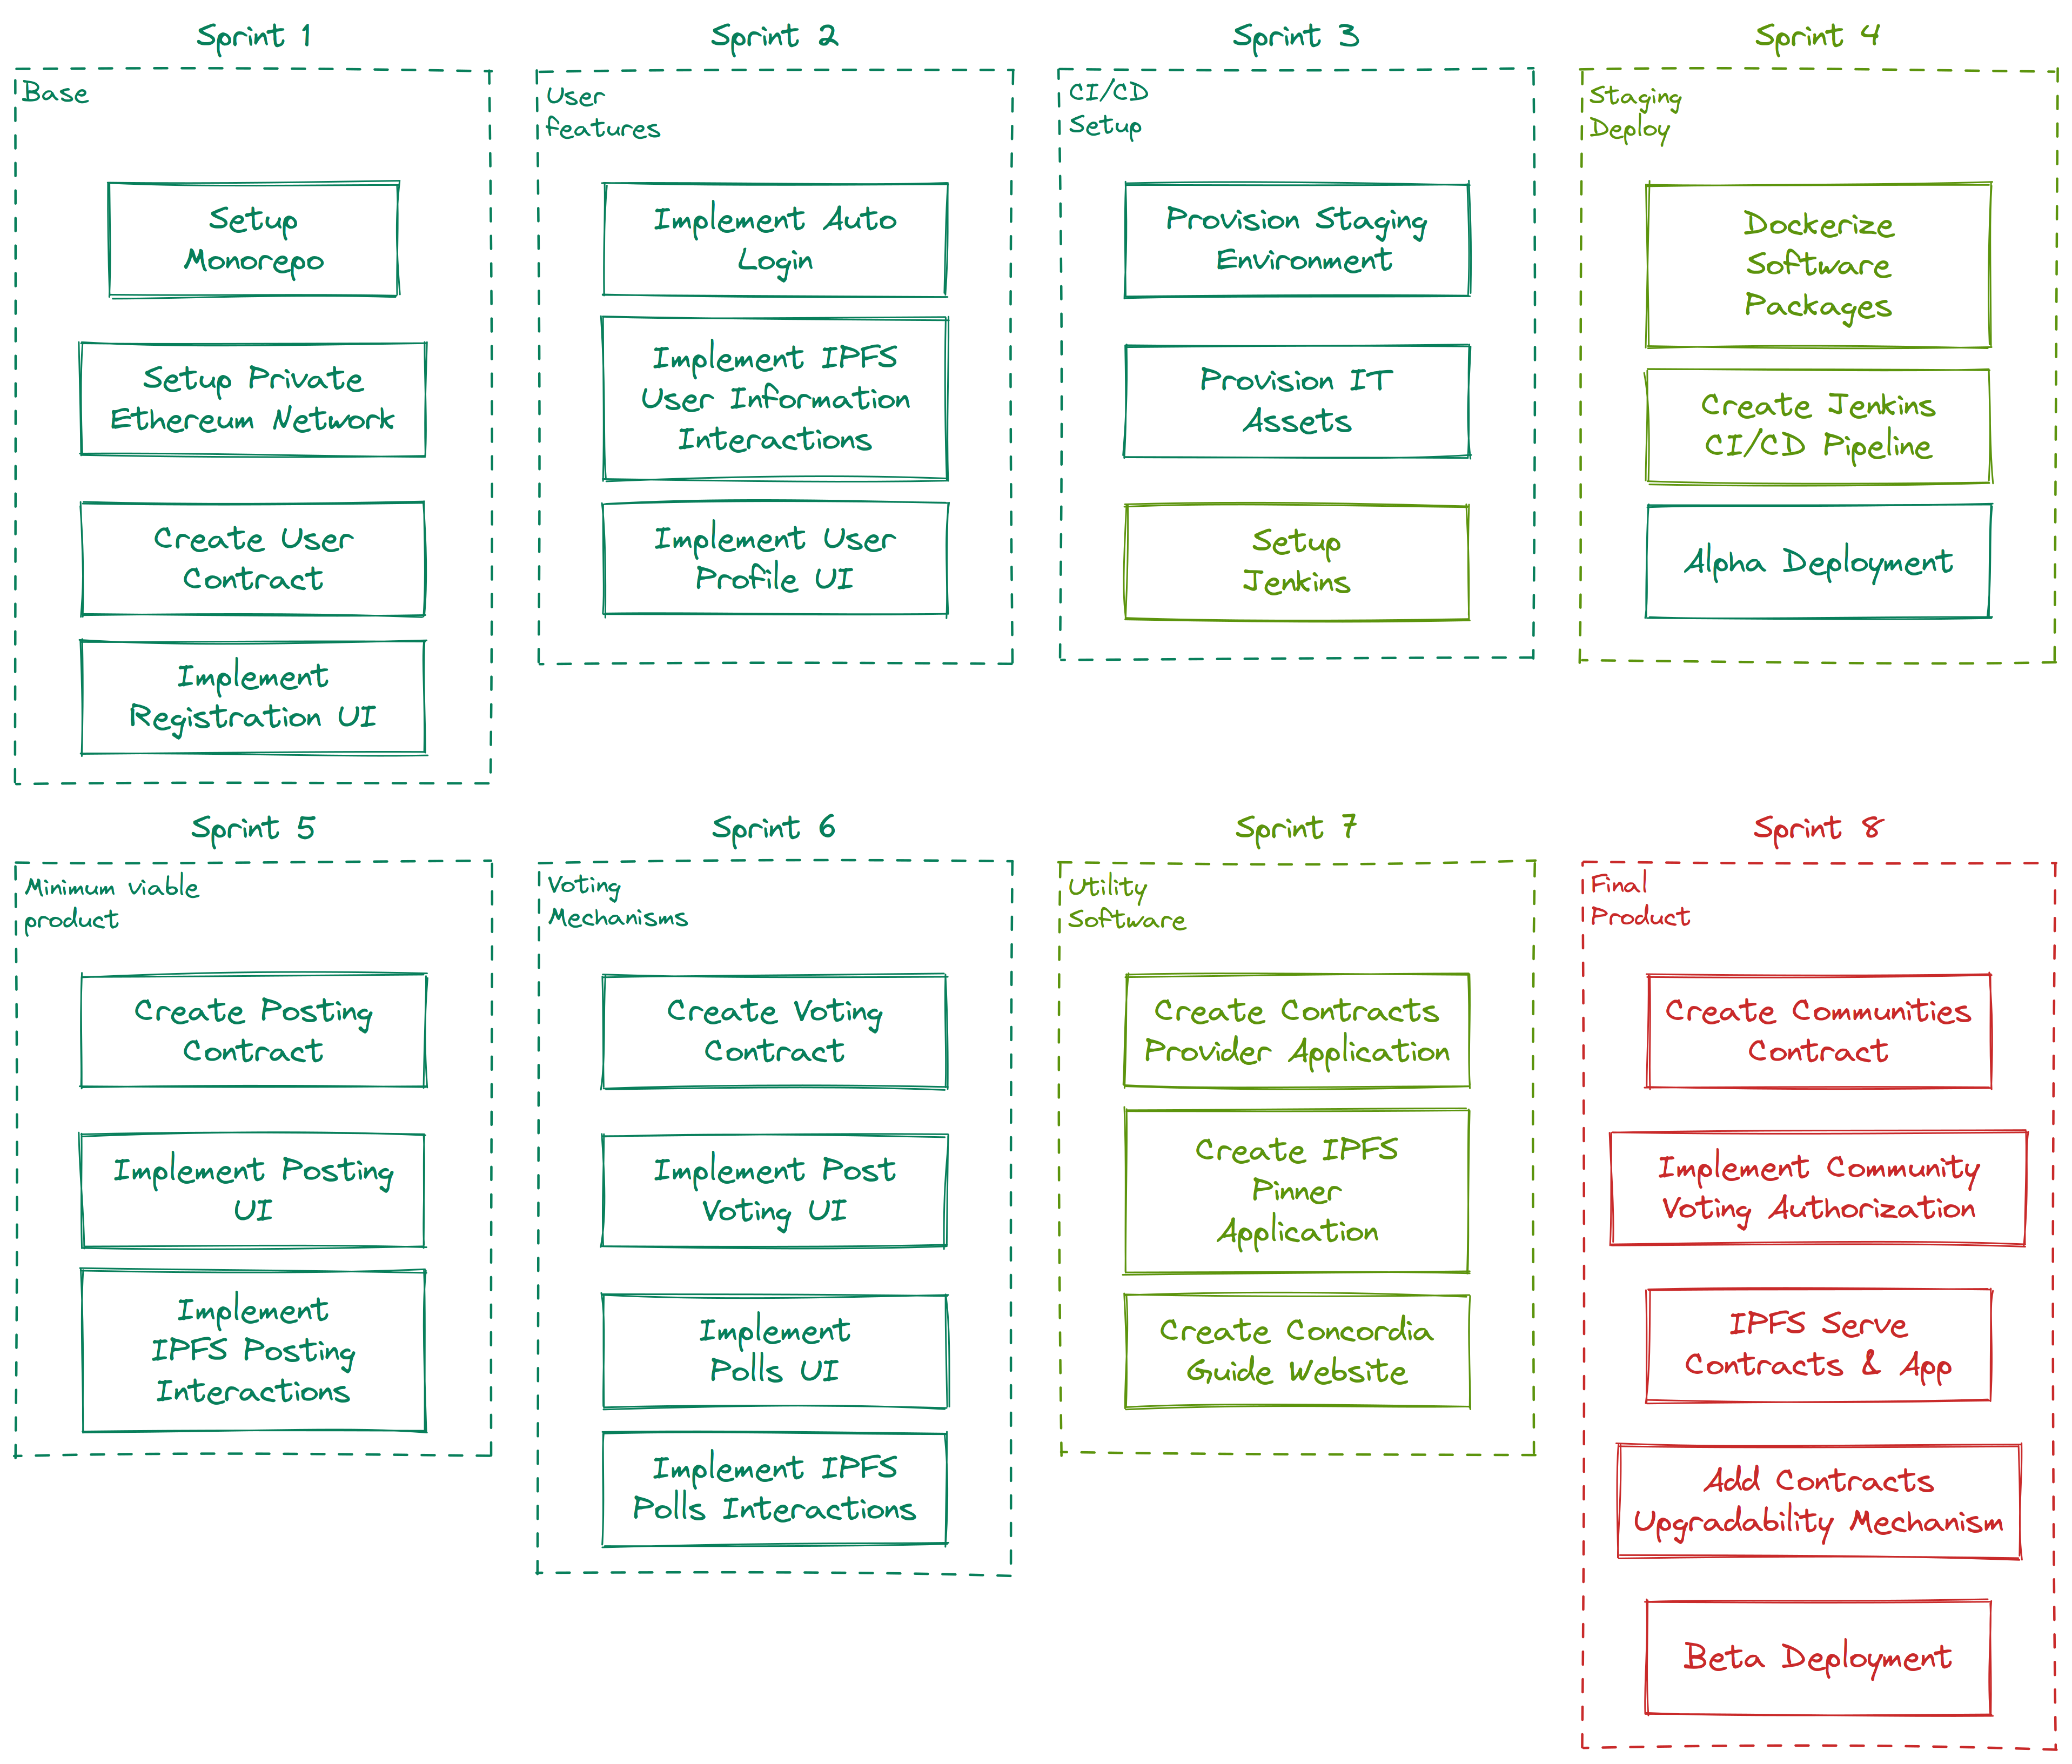
\includegraphics[width=\textwidth]{assets/figures/chapter-4/4.6.design-implementation-differences-sprints.png}
    \caption{Διαχωρισμός σε sprints}
    \label{figure:4.5.design-implementation-differences-sprints}
\end{figure}
